\documentclass[11pt,a4paper]{report}
\usepackage{ifpdf}
\usepackage[utf8]{inputenc}
\usepackage[francais]{babel}
\usepackage[french]{varioref} 
\usepackage[pdftex]{graphicx}
\usepackage{listings}
\usepackage{color}
\usepackage{amssymb}
\usepackage{amsmath}

%\usepackage{floatflt}
\usepackage{lscape} %afficher une partie en paysage


%%% Pour du code source %%%%
 \definecolor{colKeys}{rgb}{0.5,0,0.33} 
 \definecolor{colIdentifier}{rgb}{0.16,0,1} 
 \definecolor{colComments}{rgb}{0.25,0.5,0.37} 
 \definecolor{colString}{rgb}{0.6,0.1,0.1} 
 \definecolor{shadow}{rgb}{0.5,0.5,0.5} 
 
 \lstset{ 
 basicstyle=\ttfamily\small,
 identifierstyle=\color{colIdentifier},
 keywordstyle=\color{colKeys},
 stringstyle=\color{colString},
 commentstyle=\color{colComments}
 }
 \lstset{language=python}



\begin{document}

%\tableofcontents
\thispagestyle{empty}
\begin{center}
\begin{tabular}{lr}
\begin{minipage}[l]{0.4\textwidth}
\begin{flushleft}

\includegraphics[scale=0.2]{logo.png}
\end{flushleft}
\end{minipage}
&
\begin{minipage}[r]{0.4\textwidth}
\begin{flushright}
\begin{tabular}{l}
Van De Walle Bernard  (A)\\
Francois Thibault (B) \\
Van Der Essen Frédéric (C)
\end{tabular}
\end{flushright}
\end{minipage}
\end{tabular}
\end{center}

\vspace{6.5cm}

\begin{center}
\textsc{INGI2132: Langages et traducteurs}
\end{center}

\bigskip

\begin{center}
{\Huge Rapport Final}
\end{center}

\vspace{7.5cm}
\begin{center}
		\textbf{Prof.} B. Le Charlier\\
\end{center}

\vspace{1.5cm}

\newpage

\begin{figure}[h!]
\begin{center}
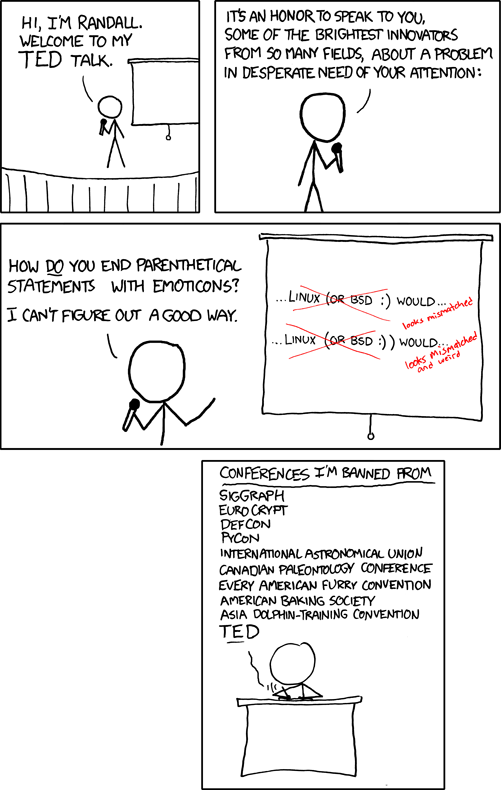
\includegraphics[scale=0.65]{xkcd.png}
\end{center}
\end{figure}
It is now possible with the HAPPY-) programming language !
\newpage


%3
\chapter{Présentation de Happy:-)}
\section{Introduction}
La langage happy, appelé ainsi parce qu'il est très permissif au niveau des caractères permit dans les identifiants comporte de nombreuses autres particularités. Tout d'abord, le langage ressemble très fort au LISP où tout est atom ou liste.
Mais contrairement au LISP, notre langage est impératif et orienté objet. Un programme est une liste de méthode, une méthode est une liste dont le premier élément est le mot réservé fun le second une list d'argument et le dernier une liste de commande. Même principe pour le while et le if. Dans ce langage tout est fonction, dans le sens que toute instruction renvoie une valeur, y compris les if et le while qui renvoient 0, une fonction qui n'a pas d'instruction return renvoie null, le write renvoie la valeur qu'elle vient d'imprimer etc...



Les conditions aurait aussi renvoyé une valeur si le langage SLIP dans lequel notre langage est traduit le permettait. 

\section{Grammaire de départ}
Cette grammaire est la grammaire exhaustive du langage si on rajoute que les id peuvent être formé de tout les caractères UTF-16 sauf des caractères réservés et qu'ils ne doivent pas être égale à un mot réservé.

\begin{verbatim}
<Program> ::= ( <Prog_list> )
<Prog_list> ::=  <Meth_or_fun> | <Prog_list> <Meth_or_fun>	
<Meth_or_fun> ::=  <Method> | <Function>

<Function> := ( fun ( <Arglist> ) <Instr_list> ) 
<Arglist> ::=  id | id <Arglist>
<Method> ::= ( <Method_int> ( <Arglist> ) <Instr_list> )
 
<Instr_list> ::=  <Instr> | ( <Instr_list_np> ) 
<Instr_list_np> ::=  <Instr> | <Instr> <Instr_list_np>
<Instr> ::=  <Conditional> | <While_block> | <Call> | ( return <Expr> ) 

<Conditional> ::= ( if <Cond> <instr_list> <instr_list>  )  
<Conditional> ::= ( if <Cond> <instr_list> )
<While_block> ::= ( while  <Cond> <Instr_list>  ) 
<call> ::=  <User_call> | <Method_call> | <Builtin_call> 
<Builtin_call> ::=  <Assignment> | <Read_call> | <Write_call> | <Arithmetic_call>
<Assignment> ::= ( set id <Expr> ) 
<Assignment> ::= ( set <Id_int> <Expr> ) | ( set <This_int> <Expr> )
<Read_call>  ::= ( read )
<Write_call> ::= ( write <Expr> )
<Arithmetic_call> ::=  <Binary> | <Unary>
<Binary> ::= ( <Bin_id> <Expr> <Expr>  )
<Unary>  ::= ( <Un_id> <Expr>  )
<User_call>  ::= ( id  <Expr_list_np> ) | ( id ) 
<Expr_list_np> ::=  <Expr> | <Expr> <Expr_list_np>
<Method_call>  ::= ( <Id_id> <Expr_list_np>  ) |  ( <Id_id> )   
<Method_call>  ::= ( <Super_id>  <Expr_list_np>  ) | ( <Super_id>  )
<Method_call>  ::= ( <This_id>  <Expr_list_np>  ) | ( <This_id> )
<Expr> ::= number | null | true | false | this | id 
<Expr> ::= <Id_int> | <This_int> | <Instr>
<Cond> ::= <Rel> | ( <Log_bin_op> <Cond> <Cond> )
<Cond> ::= ( <Log_un_op> <Cond> <Cond> )
<Rel>  ::= ( <Rel_op> <Expr> <Expr> ) 
<Rel_op> ::= <= | >= | > |  < | =
<Log_bin_op> ::= and | or
<Log_un_op> ::= !
<Bin_id> ::= + | - | * | / | %
<Un_id> ::= neg
<Id_int> ::= id . number
<This_int> ::= this . number
<Super_id> ::= super . id
<This_id> := this . id 
<Id_id> ::= id . id
<Method_int> ::= method . number
\end{verbatim}
Cette grammaire n'est pas wp, mais elle exprime très bien ce qui est syntaxiquement correcte dans ce que nous avons réellement implémenté. 

Voici quelque bout de code permis par cette grammaire :

\begin{verbatim}
[Le while s'écrit comme ceci while (la condition) (les instruction a répèter)
  ici la condition est 3 * i <= 9
On remarque aussi que sur ce bout de code on peut écrire 
la valeur de retour de set qui sera ici i_initial + 1 ou i_final ]
(while (<= (* 3  i) 9) (write (set i (+ i 1)))) 
  
[Condition ici si i != 9 ]
[Ensuite si vrai on exécute la première list d'instruction sinon la seconde]
(if (! (= i 9)) (return true) (return false))
[Ceci est équivalent à sauf que dans le cas deux on voit clairement les listes d'instructions]
(if (! (= i 9)) ((return true)) ((return false)))

(fun (++ i) (return (+ i 1)))

(set i (++ i))

(set a (new 2))
\end{verbatim}

\section{Exemple de programme complet}
Le premier programme imprime juste l'entier lu à la console.

\begin{verbatim}
(
  (fun (main) 
    (write (read))
  )
)
\end{verbatim}

Le programme suivant fait la somme de 1 à n pour 10 n
\begin{verbatim}
(
  [Programme fait la somme de 1 à n pour n qui va de 0 à 10]
  (fun (main) (
    (set i 0)
    (while (<= i 10)
    (
      (write (sum i))
      (set i (+ i 1))
    ))
  ))


  (fun (sum n) (
    (if (= n 0)
      (return 0)
    )
    (return (+ n (sum (- n 1))))
  ))
)

\end{verbatim}



Le dernier programme fait la somme des éléments d'une pile et utilise la POO
\begin{verbatim}
(
  (fun (main) (
    (set s ( >> 4 ( >> 3 (>> 2 (# 1)))))
    (write (s.@))
    (write (s.->))
    (set s (>> 5 s))
    (Print s)
    (write (sum s))
  ))
  [crée une nouvelle pile avec a comme élément au sommet]
  (fun (# a) (
    (set b (new 2))
    (b.@= a)
    (b.->= null)
    (return b)
  ))

  [Push sur la stack]
  [a : l'élément à mettre sur la stack]
  [s : la stack]
  (fun (>> a s) (
    (set n (new 2))
    (n.->= s)
    (n.@= a)
    (return n)
  )) 

  (fun (Print N) (
    (if (! (= N null)) (
      (write (N.@))
      (Print (N.->))
    )
    (write 0)
    )
  ))

  (fun (sum N) (
    (if (! (= N null)) 
      (return (+ (N.@) (sum (N.->))))
      (return 0)
    )
     
  ))
  [Accesseur pour l'élément contenu dans le noeud]
  (method.2 (@) (return this.1))
  ((method.2 (@= a) (set this.1 a))
  [Accesseur pour next]
  (method.2 (->) (return this.2))
  (method.2 (->= a) (set this.2 a))
)
\end{verbatim}




 
%7
\section{Traduction du programme en code interne}
\subsection{Création de l'arbre syntaxique du programme}
L'arbre syntaxique est consitué de \emph{Term} afin
qu'il puisse être généré directement par l'analyseur syntaxique. 
La méthode getChildList() de la classe Term renvoie la liste des \emph{Term} enfants.


Le code de l'analyser syntaxique prend en entrée un flux Term qui sont tous terminaux. 
L'analyseur syntaxique n'a besoin que des méthodes définie dans l'interface Term pour construire l'arbre.
Voici cette interface : 
\begin{verbatim}
 
\end{verbatim}
public interface Term {
	  /**
	  * 
	  * @return true if the term is a terminal term
	  */
	  public boolean isTerminal();
	  
	  /**
	  * 
	  * @return Le type du term pour l'analyseur syntaxique.
	  */
	  public String getType();
	
	  /**
	  * 
	  * @return la valeur du term, c'est à dire la chaine de caractère
	  * parsée par l'analyseur lexical.
	  * Si le term n'est pas terminal, il n'a pas de valeur
	  */
	  public String getValue();
	
	  /**
	  * Modifie la valeur du term
	  * @param v la nouvelle valeur du term
	  * @return this
	  */
	  public Term setValue(String v);
	
	  /**
	  * Renvoie la liste des enfants du terme, cette liste n'est pas vide que
	  * si le term n'es pas terminal
	  * @return
	  */
	  public List<Term> getChildList();
	
	  /**
	  * Imprime l'arbre qui est représenté par le term
	  * Indent définit le niveau d'indentation, lorsqu'on imprime
	  * l'arbre entier le point de départ est 0
	  * @param indent
	  */
	  void	printTree(int indent);
	
	
}
\end{verbatim}


Une fois le code déjà donné dans le chapitre 6 exécuté, l'arbre (le Term) passe dans le treeOrganiser.

La première chose à faire avec l'arbre généré par l'arbre brut est
de mettre tout ce qui est au même niveau de parenthèses au même niveau
dans l'arbre. Pour cela on le parcourt et on fusionne récursivement tous
les $l\_blocks$ et les $l\_lists$ dans leurs parents. Comme les \emph{Term}
gardent en mémoire le type donné à l'analyse syntaxique, les terminaux
récupèrent automatiquement le bon type. 
 
\begin{figure}
 \centering
 \includegraphics[bb=0 0 428 264]{./restruc.png}
 % restruc.png: 428x264 pixel, 72dpi, 15.10x9.31 cm, bb=0 0 428 264
 \caption{Schema simplifié de la restructuration de l'arbre}
 \label{restruc}
\end{figure}


Voici la spécification de la seul méthode public du \textit{TreeOrganiser} :
\begin{verbatim}
 /**
  * Contracte l'arbre sortit par l'analyseur syntaxique. Tout les l_list et l_block sont
  * retiré, à la fin il ne reste que des l0 qui sont soit des terminaux ou des listes de l0.
  * @return L'arbre représenté sous la forme d'un lexicalTerm
  */
public LexicalTerm contract()
\end{verbatim}

La structure de donnée LexicalTerm est très similaire à Term, elle implémente l'interface on a rajouté une méthode getLexicalTerm
qui est le type donnée par le parser lexical. Ces types ont été listé dans la partie sur l'analyseur lexical. Une fois 
l'arbre mis en forme et les types des termes réels révélés (pas ceux juste présent pour construire l'arbre), on passe à la traduction.

\section{traduction}
Il y a trois grande famille de traduction, la traduction des définitions de méthode, la traduction des instructions et la traduction des conditions.
La traduction des définitions de méthode est assez facile car on sait qu'un programme en Happy est une liste de méthode. Donc les enfants
de la racine sont les méthodes, l'enfant 0 de l'enfant est le mot clé, l'enfant 1 sont les paramètres et l'enfants 2 est la suite d'instruction.
\begin{verbatim}

/**
	 * Point de départ de l'exploration de l'arbre. 
	 * t est un term qui une liste de term qui est en accord avec la définition
	 * des méthodes ou des fonctions.
	 * Si t n'est pas conforme aux définitions, une erreur de syntaxe est lancée et le programme
	 * se termine
	 * @param t 
	 * @return la Cmethod 
	 */
	private Cmethod analyseMethod(LexicalTerm t) { 

 
\end{verbatim}

Une fois les arguments et le nom de la méthode récupéré il faut commencé à ajouté toutes les instructions à au corps de la méthode.
La méthode privée addBody crée une liste vide qui accueillera toutes les instructions de la méthode. Cette table permet de placer en premier
les instructions qui se trouvent au fond de l'arbre pour gérer correctement les appels imbriqués.

Les instructions dans le langage Happy sont toutes des expressions, c'est-à-dire qu'elle renvoie une valeur. Contrètement dans la traduction
cela ce fait par l'assignation d'une valeur (qui dépend du type d'instruction) variable annonyme qui sera renvoyé à la méthode appelante. Cette méthode
appelante utilisateur la variable si elle en a besoin.

Voici un petit exemple qui sera plus parlant :

Considérons le code Happy suivant :
\begin{verbatim}
(write 
  (set a 
    (+ 7 8)
  )
)
sera traduit en:
A_0 = 7 ; //l'expression 7 est assignée à A_0
A_1 = 8 ; //idem pour 8
A_2 = (A_0 + A_1) ; //l'expression (+ A_0 A_1) est assignée à A_2
a = A_2 ; //assignation de l'expression (+ A_0 A_1) à a en passant par A_2
A_3 = a ; //set renvoie la variable qu'il vient d'assigner
write(A_3) ;

\end{verbatim}

Les conditions fonctionne un peu comme l'exploration 

%TODO


%10
\chapter{Mode d'emploi du compilateur}
La version exécutable du compilateur et interpréteur Happy se trouve dans le jar exécutable \textit{happy.jar}.
Il prend 2 arguments obligatoire : la grammaire au format BNF et le programme en langage Happy. On peut rajouter \textit{check} à la fin pour vérifier la grammaire en plus.
Pour faire fonctionner les programmes Happy, il faut passer la grammaire \textit{temp.bnf}. Pour vérifier n'importe quelle grammaire WP, il faut indiquer la grammaire
un fichier programme bidon et enfin check.
exemple : \begin{verbatim}
    java -jar happy.jar temp.bnf programme1.happy 
    java -jar happy.jar temp.bnf programme1.happy check
          \end{verbatim}

L'interpréteur sort les informations suivantes dans cet ordre, si le check de la grammaire est demandé, le résultat des tests et la table de précédence.
Ensuite l'arbre sortit par le parser syntaxique après sa restructuration, ensuite la traduction de l'arbre en SLIP et puis (mais il semble que
les retour à la ligne ne soit pas conforme ce qui donne des résultats étranges à la sortie dans le shell) la représentation en code interne SLIP. Et finalement
la sortie du programme interprèté. 


\section{Les erreurs}
Lorsqu'une erreur arrive dans n'importe quelle partie du compilateur l'erreur est affichée (avec plus ou moins de précision) et il s'arrête ensuite.
\section{Les erreurs du vérificateur}
  

\section{Les erreurs du parser lexical}
  Il ne vérifie que deux choses. A la fin de l'analyse si il n'y a pas le même nombre de paranthèse ouvrantes que fermantes, l'erreur \textit{Unexpected end}.
  Il est aussi capable de vérifier si à tout moment il y a trop de paranthèse fermantes, le messages est dès lors très explicite : \textit{Too much ) }.
\section{Les erreurs de l'analyseur syntaxique}
  L'analyseur syntaxique signale trois erreurs. Lorsque deux termes ne peuvent se retrouver côte à côte, lorsqu'il n'arrive pas à trouver une règle pour réduire.


Et lorsqu'il a lu tout les caractères, si il reste plus d'un élément dans la pile une erreur est aussi renvoyé.
\section{Les erreurs du traducteur}
    Les erreurs que renvoient le traducteur sont d'ordre sémantique. Le programme est valide syntaxiquement mais comme notre grammaire permet beaucoup de chose,
Il faut remettre les choses en places avec le traducteur. Les erreurs sont du type : quelquechose est attendu dans ce type d'expr et là c'est pas le cas. 
exemple : textit{Expected id after a set}


\section{Les erreurs de l'interpréteur}
  L'interpréteur reporte les erreurs d'exécutions telles que la division par 0, l'appel à méthode inconnue etc...
  Les erreurs sont clairement identifié dans le code interne structurée et reporté jusqu'au dessus de la pile d'exécution. Cela permet de retracer l'erreur
sans trop de difficulté. 
Voici un exemple : 
\begin{verbatim}
Error divide by 0
	 in Cexpr a#1 / b#2
	 at Ass A_0#3 := a#1 / b#2
	 at CmdStmt [ lab9 : A_0#3 := a#1 / b#2 ; go to lab8]
	 at divide/-1
	 at Call divide
	 at CmdStmt [ lab2 : A_0#3 := divide(#4, #5) ; go to lab1]
	 at main/-1
\end{verbatim}

\end{document}
